\documentclass{report}

\usepackage[a4paper,margin=1in,landscape]{geometry}
\usepackage{array}
\usepackage{xcolor}
\usepackage{graphicx}

\newcolumntype{P}[1]{>{\raggedleft\arraybackslash}b{#1}}
\newcommand{\bftab}{\fontseries{b}\selectfont}

\begin{document}
\section{Histograms of attributes using different binning functions}

\subsection{fixed acidity}
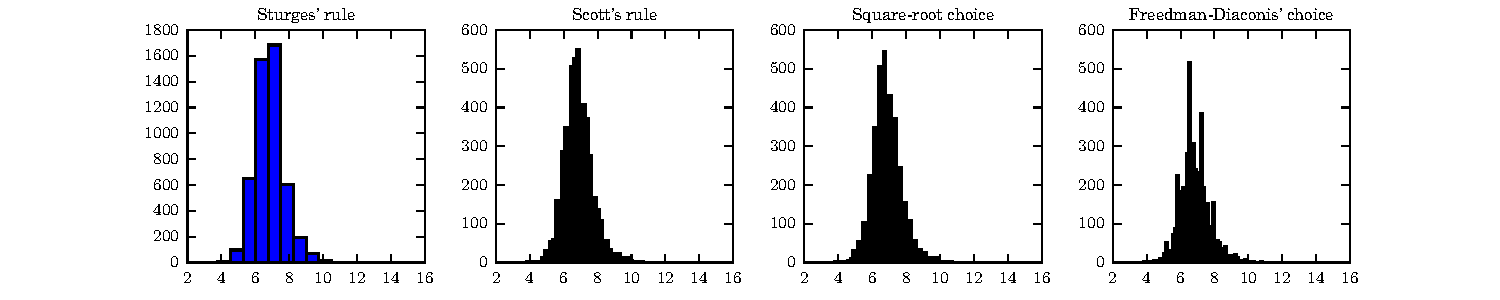
\includegraphics{histograms/fixed_acidity.pdf}

\subsection{sulphates}
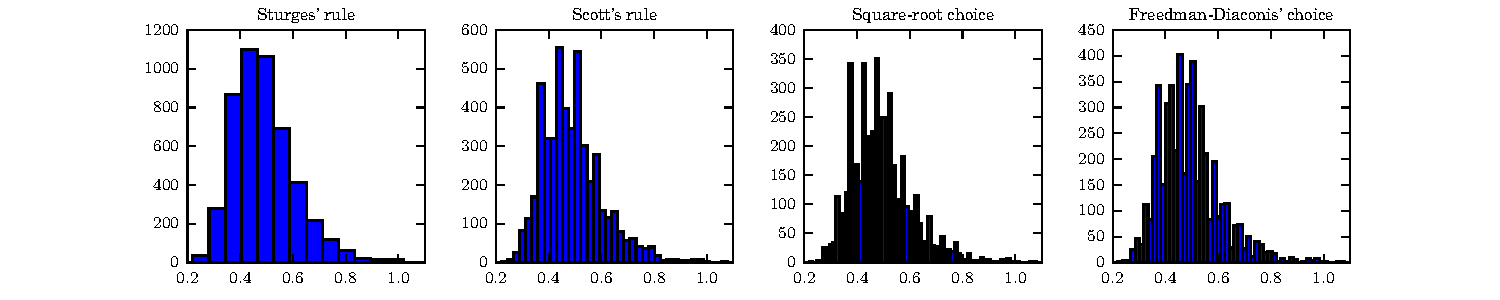
\includegraphics{histograms/sulphates.pdf}

\subsection{quality}
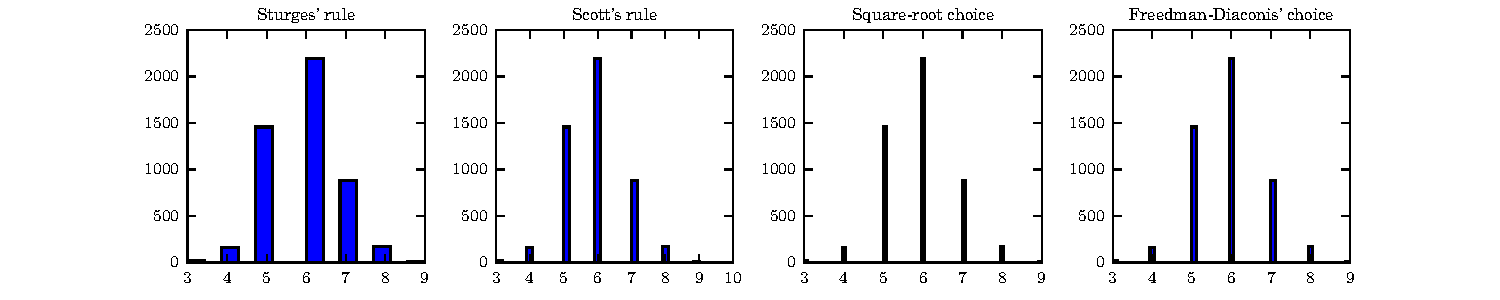
\includegraphics{histograms/quality.pdf}

\subsection{total sulfur dioxide}
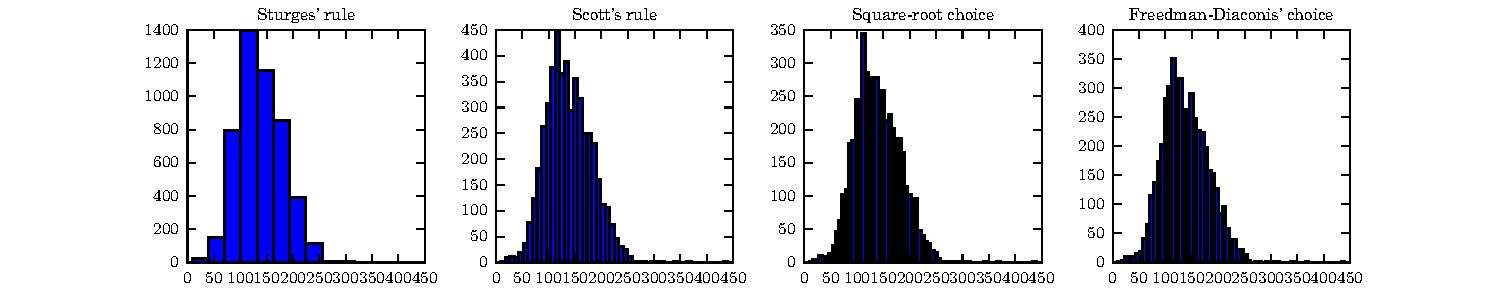
\includegraphics{histograms/total_sulfur_dioxide.pdf}

\subsection{citric acid}
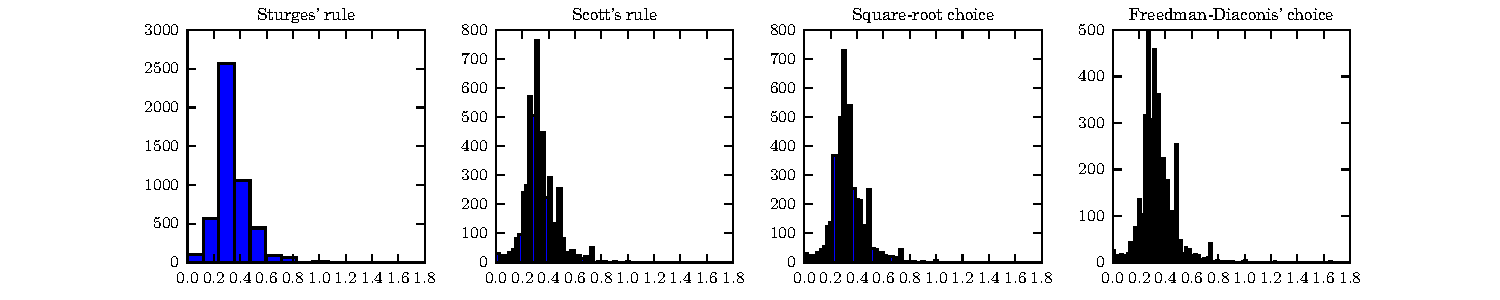
\includegraphics{histograms/citric_acid.pdf}

\subsection{residual sugar}
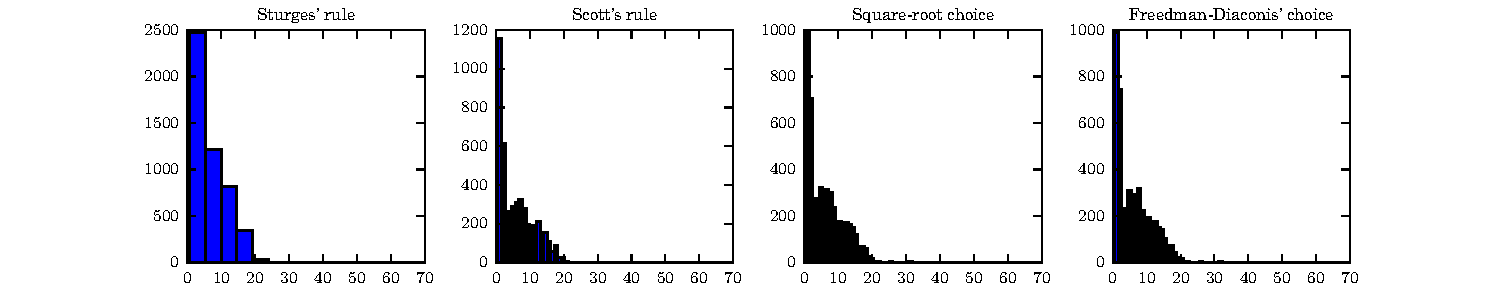
\includegraphics{histograms/residual_sugar.pdf}

\subsection{chlorides}
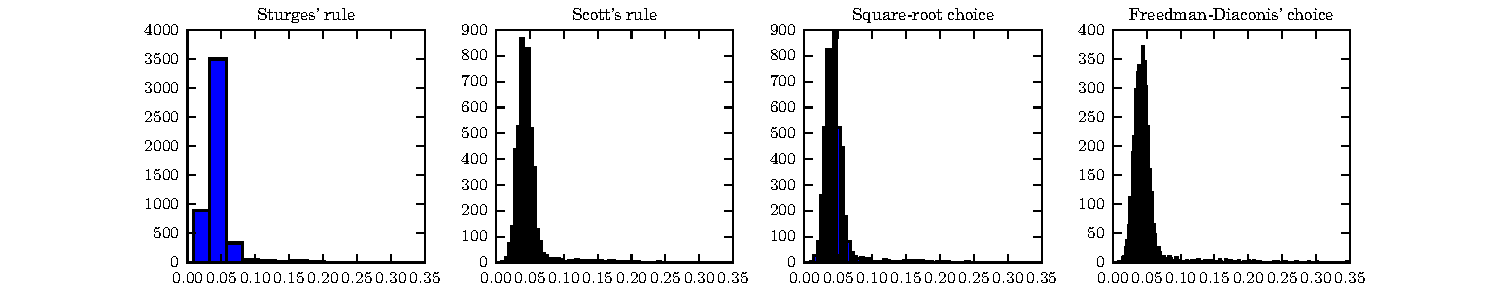
\includegraphics{histograms/chlorides.pdf}

\subsection{alcohol}
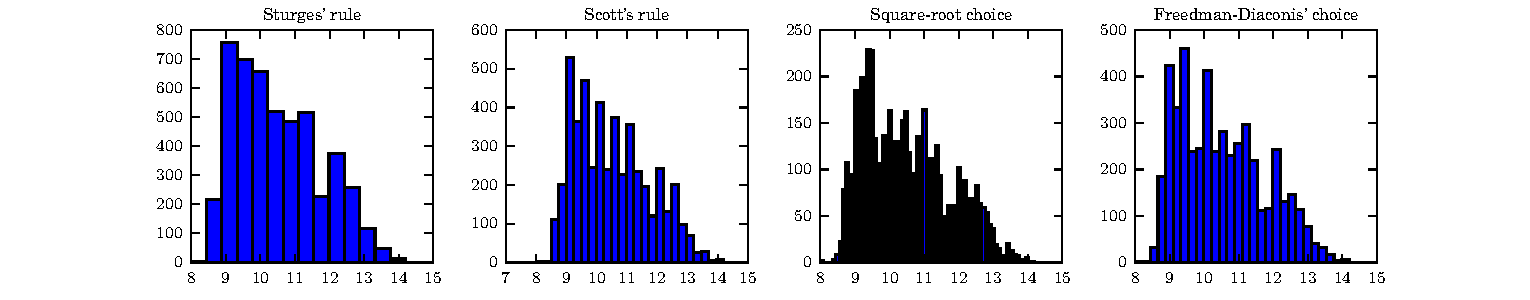
\includegraphics{histograms/alcohol.pdf}

\subsection{density}
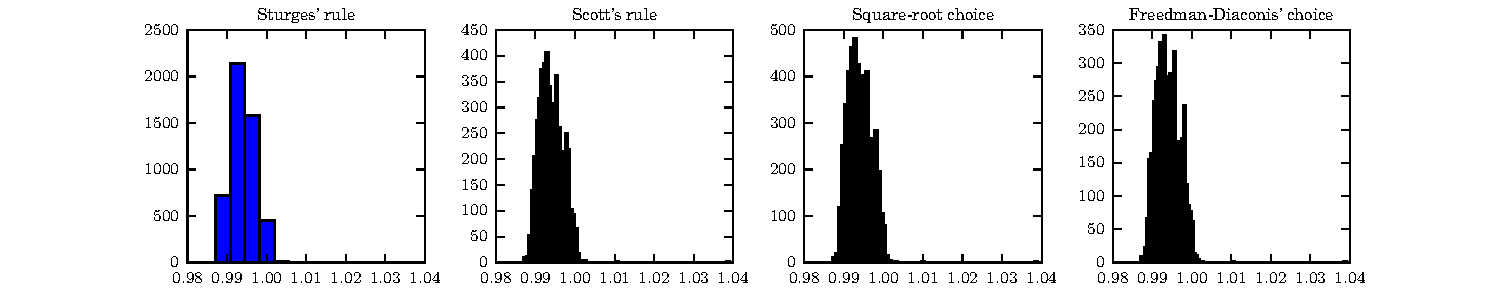
\includegraphics{histograms/density.pdf}

\subsection{free sulfur dioxide}
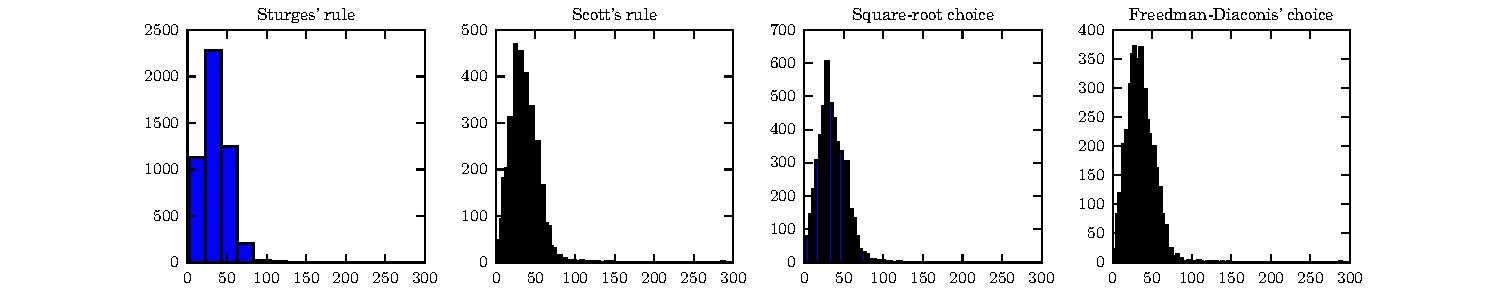
\includegraphics{histograms/free_sulfur_dioxide.pdf}

\subsection{pH}
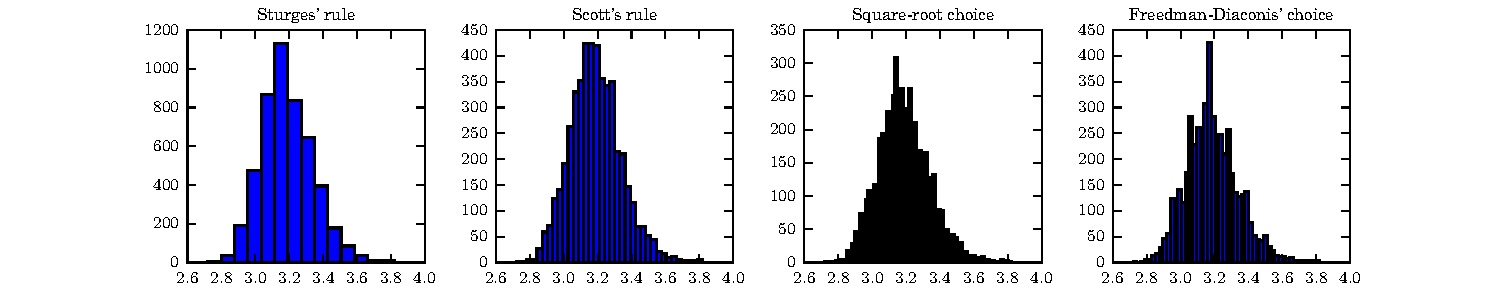
\includegraphics{histograms/pH.pdf}

\subsection{volatile acidity}
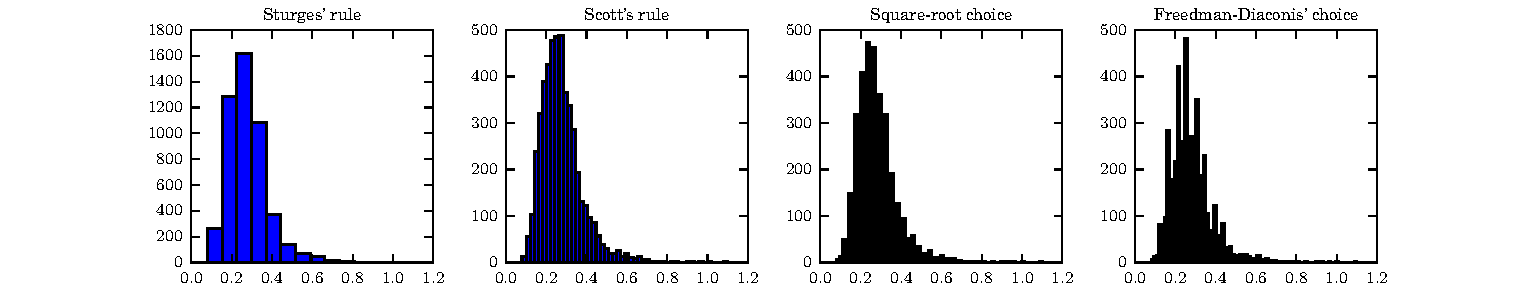
\includegraphics{histograms/volatile_acidity.pdf}

\section{Correlation coefficients using different functions}

\subsection{Correlation coefficients using Pearson's correlation coefficient}
\begin{tabular}{l || *{12}{P{1.2cm}}}
& fixed acidity & sulphates & quality & total sulfur dioxide & citric acid & residual sugar & chlorides & alcohol & density & free sulfur dioxide & pH & volatile acidity\\
\hline 
fixed acidity & \bftab 1.0000 & -0.0171 & -0.1137 & 0.0911 & 0.2892 & 0.0890 & 0.0231 & -0.1209 & 0.2653 & -0.0494 & -0.4259 & -0.0227 \\

sulphates & -0.0171 & \bftab 1.0000 & 0.0537 & 0.1346 & 0.0623 & -0.0267 & 0.0168 & -0.0174 & 0.0745 & 0.0592 & 0.1560 & -0.0357 \\

quality & -0.1137 & 0.0537 & \bftab 1.0000 & -0.1747 & -0.0092 & -0.0976 & -0.2099 & 0.4356 & -0.3071 & 0.0082 & 0.0994 & -0.1947 \\

total sulfur dioxide & 0.0911 & 0.1346 & -0.1747 & \bftab 1.0000 & 0.1211 & 0.4014 & 0.1989 & -0.4489 & \bftab 0.5299 & \bftab 0.6155 & 0.0023 & 0.0893 \\

citric acid & 0.2892 & 0.0623 & -0.0092 & 0.1211 & \bftab 1.0000 & 0.0942 & 0.1144 & -0.0757 & 0.1495 & 0.0941 & -0.1637 & -0.1495 \\

residual sugar & 0.0890 & -0.0267 & -0.0976 & 0.4014 & 0.0942 & \bftab 1.0000 & 0.0887 & -0.4506 & \bftab 0.8390 & 0.2991 & -0.1941 & 0.0643 \\

chlorides & 0.0231 & 0.0168 & -0.2099 & 0.1989 & 0.1144 & 0.0887 & \bftab 1.0000 & -0.3602 & 0.2572 & 0.1014 & -0.0904 & 0.0705 \\

alcohol & -0.1209 & -0.0174 & 0.4356 & -0.4489 & -0.0757 & -0.4506 & -0.3602 & \bftab 1.0000 & \bftab -0.7801 & -0.2501 & 0.1214 & 0.0677 \\

density & 0.2653 & 0.0745 & -0.3071 & \bftab 0.5299 & 0.1495 & \bftab 0.8390 & 0.2572 & \bftab -0.7801 & \bftab 1.0000 & 0.2942 & -0.0936 & 0.0271 \\

free sulfur dioxide & -0.0494 & 0.0592 & 0.0082 & \bftab 0.6155 & 0.0941 & 0.2991 & 0.1014 & -0.2501 & 0.2942 & \bftab 1.0000 & -0.0006 & -0.0970 \\

pH & -0.4259 & 0.1560 & 0.0994 & 0.0023 & -0.1637 & -0.1941 & -0.0904 & 0.1214 & -0.0936 & -0.0006 & \bftab 1.0000 & -0.0319 \\

volatile acidity & -0.0227 & -0.0357 & -0.1947 & 0.0893 & -0.1495 & 0.0643 & 0.0705 & 0.0677 & 0.0271 & -0.0970 & -0.0319 & \bftab 1.0000 \\
\end{tabular}

\subsection{Correlation coefficients using Spearman's rho}
\begin{tabular}{l || *{12}{P{1.2cm}}}
& fixed acidity & sulphates & quality & total sulfur dioxide & citric acid & residual sugar & chlorides & alcohol & density & free sulfur dioxide & pH & volatile acidity\\
\hline 
fixed acidity & \bftab 1.0000 & -0.0132 & -0.0845 & 0.1126 & 0.2979 & 0.1067 & 0.0947 & -0.1068 & 0.2700 & -0.0245 & -0.4183 & -0.0429 \\

sulphates & -0.0132 & \bftab 1.0000 & 0.0333 & 0.1578 & 0.0798 & -0.0038 & 0.0939 & -0.0449 & 0.0951 & 0.0523 & 0.1402 & -0.0169 \\

quality & -0.0845 & 0.0333 & \bftab 1.0000 & -0.1967 & 0.0183 & -0.0821 & -0.3145 & 0.4404 & -0.3484 & 0.0237 & 0.1094 & -0.1966 \\

total sulfur dioxide & 0.1126 & 0.1578 & -0.1967 & \bftab 1.0000 & 0.0932 & 0.4313 & 0.3752 & -0.4766 & \bftab 0.5638 & \bftab 0.6186 & -0.0118 & 0.1176 \\

citric acid & 0.2979 & 0.0798 & 0.0183 & 0.0932 & \bftab 1.0000 & 0.0246 & 0.0327 & -0.0292 & 0.0914 & 0.0883 & -0.1462 & -0.1504 \\

residual sugar & 0.1067 & -0.0038 & -0.0821 & 0.4313 & 0.0246 & \bftab 1.0000 & 0.2278 & -0.4453 & \bftab 0.7804 & 0.3461 & -0.1800 & 0.1086 \\

chlorides & 0.0947 & 0.0939 & -0.3145 & 0.3752 & 0.0327 & 0.2278 & \bftab 1.0000 & \bftab -0.5708 & \bftab 0.5083 & 0.1670 & -0.0540 & -0.0049 \\

alcohol & -0.1068 & -0.0449 & 0.4404 & -0.4766 & -0.0292 & -0.4453 & \bftab -0.5708 & \bftab 1.0000 & \bftab -0.8219 & -0.2726 & 0.1489 & 0.0340 \\

density & 0.2700 & 0.0951 & -0.3484 & \bftab 0.5638 & 0.0914 & \bftab 0.7804 & \bftab 0.5083 & \bftab -0.8219 & \bftab 1.0000 & 0.3278 & -0.1101 & 0.0101 \\

free sulfur dioxide & -0.0245 & 0.0523 & 0.0237 & \bftab 0.6186 & 0.0883 & 0.3461 & 0.1670 & -0.2726 & 0.3278 & \bftab 1.0000 & -0.0063 & -0.0812 \\

pH & -0.4183 & 0.1402 & 0.1094 & -0.0118 & -0.1462 & -0.1800 & -0.0540 & 0.1489 & -0.1101 & -0.0063 & \bftab 1.0000 & -0.0452 \\

volatile acidity & -0.0429 & -0.0169 & -0.1966 & 0.1176 & -0.1504 & 0.1086 & -0.0049 & 0.0340 & 0.0101 & -0.0812 & -0.0452 & \bftab 1.0000 \\
\end{tabular}

\subsection{Correlation coefficients using Kendall's tau}
\begin{tabular}{l || *{12}{P{1.2cm}}}
& fixed acidity & sulphates & quality & total sulfur dioxide & citric acid & residual sugar & chlorides & alcohol & density & free sulfur dioxide & pH & volatile acidity\\
\hline 
fixed acidity & \bftab 1.0000 & -0.0087 & -0.0655 & 0.0773 & 0.2086 & 0.0749 & 0.0654 & -0.0732 & 0.1855 & -0.0169 & -0.2948 & -0.0296 \\

sulphates & -0.0087 & \bftab 1.0000 & 0.0264 & 0.1087 & 0.0545 & -0.0025 & 0.0626 & -0.0264 & 0.0642 & 0.0356 & 0.0958 & -0.0116 \\

quality & -0.0655 & 0.0264 & \bftab 1.0000 & -0.1512 & 0.0146 & -0.0631 & -0.2449 & 0.3467 & -0.2666 & 0.0172 & 0.0844 & -0.1548 \\

total sulfur dioxide & 0.0773 & 0.1087 & -0.1512 & \bftab 1.0000 & 0.0622 & 0.2933 & 0.2571 & -0.3258 & 0.3884 & 0.4447 & -0.0084 & 0.0813 \\

citric acid & 0.2086 & 0.0545 & 0.0146 & 0.0622 & \bftab 1.0000 & 0.0153 & 0.0223 & -0.0200 & 0.0615 & 0.0608 & -0.1013 & -0.1040 \\

residual sugar & 0.0749 & -0.0025 & -0.0631 & 0.2933 & 0.0153 & \bftab 1.0000 & 0.1553 & -0.3056 & \bftab 0.5890 & 0.2367 & -0.1256 & 0.0728 \\

chlorides & 0.0654 & 0.0626 & -0.2449 & 0.2571 & 0.0223 & 0.1553 & \bftab 1.0000 & -0.4040 & 0.3491 & 0.1139 & -0.0379 & -0.0035 \\

alcohol & -0.0732 & -0.0264 & 0.3467 & -0.3258 & -0.0200 & -0.3056 & -0.4040 & \bftab 1.0000 & \bftab -0.6351 & -0.1825 & 0.1026 & 0.0235 \\

density & 0.1855 & 0.0642 & -0.2666 & 0.3884 & 0.0615 & \bftab 0.5890 & 0.3491 & \bftab -0.6351 & \bftab 1.0000 & 0.2173 & -0.0756 & 0.0066 \\

free sulfur dioxide & -0.0169 & 0.0356 & 0.0172 & 0.4447 & 0.0608 & 0.2367 & 0.1139 & -0.1825 & 0.2173 & \bftab 1.0000 & -0.0052 & -0.0548 \\

pH & -0.2948 & 0.0958 & 0.0844 & -0.0084 & -0.1013 & -0.1256 & -0.0379 & 0.1026 & -0.0756 & -0.0052 & \bftab 1.0000 & -0.0304 \\

volatile acidity & -0.0296 & -0.0116 & -0.1548 & 0.0813 & -0.1040 & 0.0728 & -0.0035 & 0.0235 & 0.0066 & -0.0548 & -0.0304 & \bftab 1.0000 \\
\end{tabular}

\end{document}